\documentclass[11pt,a4paper]{report}
\usepackage[utf8]{inputenc}
\usepackage[T1]{fontenc}
\usepackage[italian]{babel}
\usepackage{lmodern}
\usepackage[margin=2.6cm]{geometry}
\usepackage{graphicx}
\usepackage{booktabs}
\usepackage{siunitx}
\sisetup{output-decimal-marker={,},group-separator={.},group-minimum-digits=4,table-format=1.3}
\usepackage{caption}
\usepackage{xcolor}
\usepackage{microtype}
\usepackage[hidelinks]{hyperref}
\usepackage{float}
\usepackage{tabularx}
\newcommand{\gr}{GraphRAG}
\definecolor{grblue}{HTML}{1f5fa8}

\begin{document}

\chapter*{Scaling della profondità dei salti}
\addcontentsline{toc}{chapter}{Scaling della profondità dei salti}

\section*{Domanda sperimentale}

Fino a che punto la struttura del grafo continua a proteggere il recupero quando la catena
di ragionamento clinico si allunga? Gli esperimenti precedenti hanno lavorato su domande a
2--5 salti. Qui portiamo la profondità fino a \textbf{8 salti} e misuriamo due grandezze
distinte, entrambe in modo deterministico e offline (router = oracolo, nessun modello
linguistico nel ciclo di misura):

\begin{enumerate}
  \item \textbf{Recall del fatto terminale} --- il nome dell'entità-obiettivo finale compare
        nel contesto recuperato?
  \item \textbf{Chain-recall (completezza della catena)} --- quale frazione dei nomi-ponte
        intermedi compare nel contesto?
\end{enumerate}

La seconda metrica è il cuore di questo esperimento: una risposta a molti salti è utile non
solo se contiene il fatto finale, ma se contiene \emph{tutti gli anelli} che lo giustificano.

\section*{Disegno: una spina tipizzata, lo stesso gene ad ogni profondità}

Il rischio metodologico in un esperimento di profondità è confondere la profondità con la
scelta del sotto-grafo. Lo evitiamo con una \textbf{spina tipizzata unica}:

\begin{quote}\itshape
Gene $\rightarrow$ Variant $\rightarrow$ MolecularProfile $\rightarrow$ Evidence
$\rightarrow$ Drug $\rightarrow$ CompanionDiagnostic $\rightarrow$ Gene$'$
$\rightarrow$ Variant$'$ $\rightarrow$ MolecularProfile$'$
\end{quote}

Ogni gene-ancora che possiede un \textbf{cammino canonico completo} a profondità 8
(\num{91} geni, selezionati fra \num{1437}; visita in profondità deterministica con
successori mescolati dal seme \texttt{20240517}) viene troncato a profondità crescenti.
Poiché \textbf{lo stesso gene} genera la domanda ad ogni profondità, la profondità resta
l'unica variabile manipolata.

La profondità~3 ha come terminale un nodo \textsf{Evidence}, che nel grafo \textbf{non ha
attributo \texttt{name}}: non è nominabile in un test testuale, quindi è esclusa. Le
profondità usate sono \textbf{1, 2, 4, 5, 6, 7, 8}, per un totale di \num{637} domande
(\num{91} ancore $\times$ 7 profondità).

\section*{La covariata onesta: quanti passaggi separati servono}

Prima dei risultati documentiamo il meccanismo. La Figura~\ref{fig:fanout} conta, per
ciascun cammino canonico, quanti \textbf{passaggi distinti} del corpus servono per
testimoniare l'intera catena (un passaggio testimonia un salto se il suo testo contiene i
nomi di entrambi gli estremi). Fino alla profondità~4 la mediana è \textbf{1}: l'intera
catena vive dentro un solo passaggio ricco, perché il corpus è \emph{evidence-centric} e
un passaggio raggruppa gene, variante, profilo, evidenza e farmaco. Da profondità~5 la
mediana sale a 2, poi a 3 (profondità~7) e a 4 (profondità~8): il RAG deve
\textbf{recuperare e unire passaggi separati}, ed è lì che ci aspettiamo il crollo del
recupero testuale.

\begin{figure}[H]
  \centering
  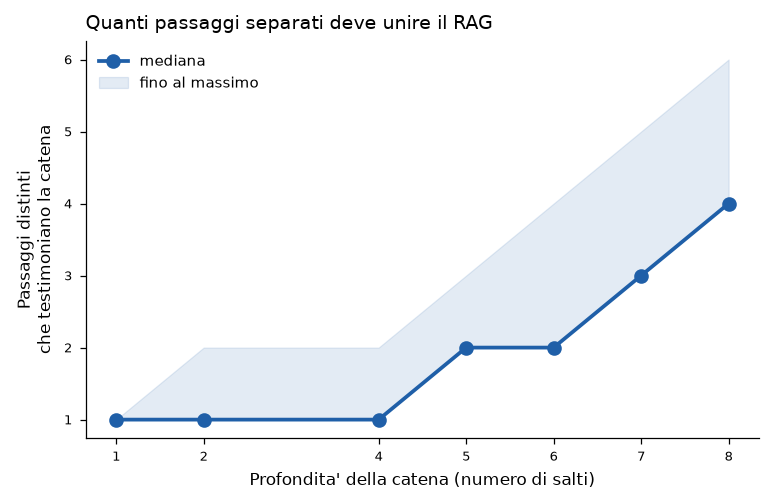
\includegraphics[width=0.62\textwidth]{deep_hops_fanout.png}
  \caption{Passaggi distinti del corpus necessari a testimoniare l'intera catena, in
  funzione della profondità. Fino a 4 salti basta un passaggio; da 5 in poi il recupero
  testuale deve unire fonti separate.}
  \label{fig:fanout}
\end{figure}

\section*{Risultati}

\begin{figure}[H]
  \centering
  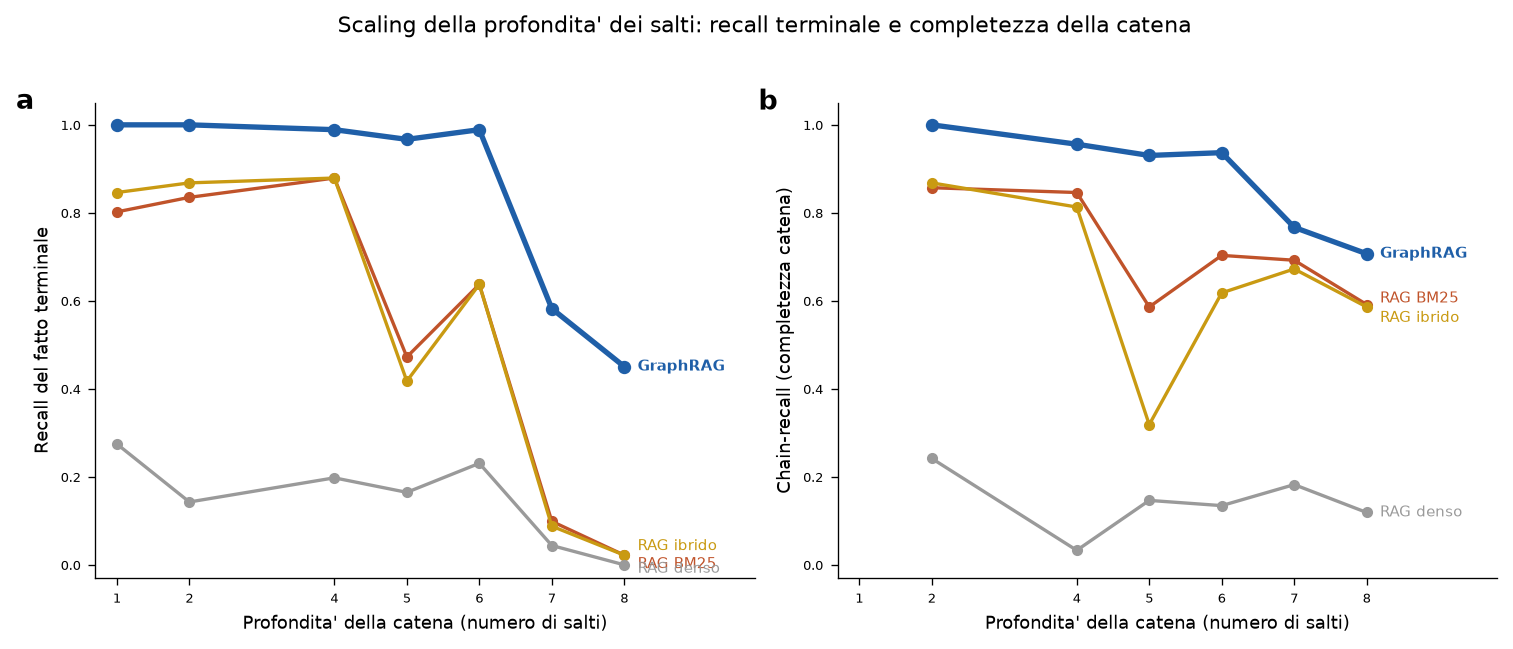
\includegraphics[width=\textwidth]{fig13_profondita_salti.png}
  \caption{Scaling della profondità dei salti. (a)~Recall del fatto terminale vs profondità.
  (b)~Chain-recall (completezza della catena) vs profondità. \gr{} (blu) è la linea focale.}
  \label{fig:fig13}
\end{figure}

\subsection*{Recall del fatto terminale}

\begin{table}[H]
  \centering
  \begin{tabular}{r S S S S}
    \toprule
    Profondità & {\gr} & {RAG BM25} & {RAG ibrido} & {RAG denso} \\
    \midrule
    1 & 1.000 & 0.802 & 0.846 & 0.275 \\
    2 & 1.000 & 0.835 & 0.868 & 0.143 \\
    4 & 0.989 & 0.879 & 0.879 & 0.198 \\
    5 & 0.967 & 0.473 & 0.418 & 0.165 \\
    6 & 0.989 & 0.637 & 0.637 & 0.231 \\
    7 & 0.582 & 0.099 & 0.088 & 0.044 \\
    8 & 0.451 & 0.022 & 0.022 & 0.000 \\
    \bottomrule
  \end{tabular}
  \caption{Recall del fatto terminale per sistema e profondità.}
\end{table}

\gr{} \textbf{domina ad ogni profondità}. Il salto~5 (Farmaco~$\rightarrow$~Test
diagnostico) è un vero scoglio per il RAG: la recall di BM25 crolla da \num{0.879} a
\num{0.473} perché il farmaco e il suo test di accompagnamento \textbf{non sono più
co-menzionati nello stesso passaggio}. \gr{}, che attraversa l'arco
\textsf{HAS\_COMPANION\_DIAGNOSTIC} esplicitamente, resta a \num{0.967}.

Il calo di \gr{} a profondità 7--8 è un \textbf{confondimento di fan-out documentato, non un
guasto}. Il settimo salto è un secondo \textsf{HAS\_VARIANT}: il gene raggiunto può
ramificare in decine di varianti. Per ABCB1 la profondità~8 genera \num{162} cammini; sotto
il budget di \num{900} parole solo circa 17 vengono serializzati, quindi lo \emph{specifico}
terminale canonico compete con i suoi fratelli e non sempre entra nel contesto. È recupero
limitato dal budget su un ventaglio combinatorio --- la stessa pressione che la covariata di
fan-out anticipa.

\subsection*{Chain-recall / completezza della catena}

\begin{table}[H]
  \centering
  \begin{tabular}{r S S S S}
    \toprule
    Profondità & {\gr} & {RAG BM25} & {RAG ibrido} & {RAG denso} \\
    \midrule
    2 & 1.000 & 0.857 & 0.868 & 0.242 \\
    4 & 0.956 & 0.846 & 0.813 & 0.033 \\
    5 & 0.930 & 0.586 & 0.319 & 0.147 \\
    6 & 0.937 & 0.703 & 0.618 & 0.135 \\
    7 & 0.767 & 0.692 & 0.673 & 0.182 \\
    8 & 0.707 & 0.592 & 0.586 & 0.119 \\
    \bottomrule
  \end{tabular}
  \caption{Chain-recall (frazione dei nomi-ponte presenti nel contesto) per sistema e
  profondità. La profondità~1 non ha ponti intermedi.}
\end{table}

Qui emerge la proprietà strutturale di \gr{}. Ogni cammino serializzato è \textbf{internamente
completo per costruzione} --- nomina tutti i nodi-ponte lungo la spina --- quindi la
chain-recall \textbf{degrada con grazia} (\num{1.000}~$\rightarrow$~\num{0.707}) invece di
crollare. Il RAG denso, che deve coprire ogni salto in modo indipendente, resta
\textbf{sotto \num{0.20}} a ogni profondità: la probabilità che un singolo recupero copra
\emph{tutti} gli anelli decade moltiplicativamente. BM25 e ibrido tengono meglio del denso
ma restano circa \num{0.12}--\num{0.15} sotto \gr{} per tutta la coda.

Si noti che a profondità 7--8 la chain-recall di \gr{} (\num{0.767} / \num{0.707}) è
\textbf{molto più alta} della sua recall terminale (\num{0.582} / \num{0.451}): anche quando
il budget espelle lo specifico terminale, gli anelli intermedi della catena restano in gran
parte nel contesto. La struttura preserva il \emph{ragionamento} anche dove il ventaglio
combinatorio mette sotto pressione la singola risposta finale.

\section*{Conclusioni}

\begin{enumerate}
  \item \textbf{La struttura protegge il recupero profondo.} Su terminale e catena, \gr{} è
        superiore ad ogni profondità; il divario si allarga proprio dove la catena smette di
        vivere in un unico passaggio (profondità $\geq 5$).
  \item \textbf{La completezza della catena è la metrica che separa i paradigmi.} \gr{}
        degrada con grazia perché ogni cammino è completo per costruzione; il RAG denso
        collassa perché deve coprire ogni salto in modo indipendente.
  \item \textbf{Il limite di \gr{} è il budget, non la connettività.} Il calo terminale a
        profondità 7--8 è ventaglio combinatorio sotto un budget fisso di \num{900} parole
        --- un limite di \emph{impaginazione}, non di \emph{raggiungibilità}: la connettività
        del grafo garantisce che il terminale sia sempre a distanza finita; è la
        serializzazione a doverlo scegliere fra molti fratelli.
\end{enumerate}

\end{document}
